\documentclass[11pt]{article}
\usepackage[notes]{la}
\lamodule{3}{1}{Introduction to Determinants}
\laxdoc{2.2}
\laxdoc{2.3}

\begin{document}

\section{Introduction to Determinants}

\begin{guide}
In Section 2.2 a single number, $ad-bc$, decided whether a $2\times2$ matrix can be undone, and its absolute value was the area of the image of the unit square. Is there a single number that does the same job for a $3\times3$ matrix, or for a $4\times4$ one? What would it have to look like? And once we have it, how can we compute it without drowning in arithmetic?
\end{guide}

\textbf{By the end of this section you should be able to:}
\begin{itemize}
  \item explain why $ad-bc$ suggests a search for a similar number for $3\times3$ matrices, and how row reduction of a general $3\times3$ matrix leads to it;
  \item find the submatrix $A_{ij}$, the minor and the cofactor $C_{ij}=(-1)^{i+j}\det A_{ij}$ of an entry, and write the checkerboard of signs for any size;
  \item compute a determinant by cofactor expansion along the first row;
  \item state the theorem that expansion along \emph{any} row or \emph{any} column gives the same number, and explain why it is true for $3\times3$ matrices;
  \item choose the row or column with the most zeros and use it to shorten a computation;
  \item compute the determinant of a triangular matrix at a glance, and recognise a matrix with a zero row or a zero column;
  \item avoid the sign errors that are typical of cofactor expansion;
  \item explain why cofactor expansion is practical only for small matrices.
\end{itemize}

% ---------------------------------------------------------------------
\subsection*{A number for $3\times3$ matrices}

By Theorem~\ref{2.2-thm:twobytwo} the matrix $\begin{bmatrix}a&b\\c&d\end{bmatrix}$ is invertible exactly when $ad-bc\neq0$, and in Section 2.2 we saw that $|ad-bc|$ is the area of the image of the unit square. In Section 2.3 invertibility of an $n\times n$ matrix turned out to have many disguises (Theorem~\ref{2.3-thm:imt}), but every disguise asks us to row reduce or to find a lucky shortcut. For $2\times2$ matrices one formula settles the question at a glance. We look for a number, computed from the nine entries of a $3\times3$ matrix, that is nonzero exactly when the matrix is invertible.

We ask row reduction what the number should be. Let $A=[a_{ij}]$ be a $3\times3$ matrix with $a_{11}\neq0$. Multiply rows $2$ and $3$ by $a_{11}$ (allowed, since $a_{11}\neq0$), and then subtract $a_{21}$ times row $1$ from the new row $2$ and $a_{31}$ times row $1$ from the new row $3$. Put
\[
p=a_{11}a_{22}-a_{12}a_{21},\quad q=a_{11}a_{23}-a_{13}a_{21},\quad r=a_{11}a_{32}-a_{12}a_{31},\quad s=a_{11}a_{33}-a_{13}a_{31}.
\]
The result is the matrix $\begin{bmatrix}a_{11}&a_{12}&a_{13}\\0&p&q\\0&r&s\end{bmatrix}$. Notice that $p$ is the $2\times2$ number of the upper left corner of $A$. If $p\neq0$, multiply row $3$ by $p$ and subtract $r$ times row $2$: the third pivot becomes $ps-qr$, and a direct computation (expand and compare) shows
\[
ps-qr=a_{11}\Delta,\qquad\text{where}\qquad
\Delta=a_{11}(a_{22}a_{33}-a_{23}a_{32})-a_{12}(a_{21}a_{33}-a_{23}a_{31})+a_{13}(a_{21}a_{32}-a_{22}a_{31}).
\]
So for $a_{11}\neq0$ and $p\neq0$ the matrix $A$ is row equivalent to a triangular matrix with diagonal entries $a_{11},\ p,\ a_{11}\Delta$. It has three pivots, and is therefore invertible (Theorem~\ref{2.3-thm:imt}), exactly when $\Delta\neq0$. The number $\Delta$ is the one we were looking for.

Look at how $\Delta$ is built. Each bracket is the $2\times2$ number of what remains of $A$ after we delete row~$1$ and one column, and the three terms carry the alternating signs $+,-,+$:
\begin{equation}\label{eq:delta}
\Delta=a_{11}\begin{vmatrix}a_{22}&a_{23}\\a_{32}&a_{33}\end{vmatrix}-a_{12}\begin{vmatrix}a_{21}&a_{23}\\a_{31}&a_{33}\end{vmatrix}+a_{13}\begin{vmatrix}a_{21}&a_{22}\\a_{31}&a_{32}\end{vmatrix}.
\end{equation}
(The vertical bars around an array of numbers mean the determinant of that array, here $ad-bc$.) A $3\times3$ determinant is built from $2\times2$ determinants. This suggests a definition that builds a $4\times4$ determinant from $3\times3$ ones, and so on.

\begin{think}{What should the number do?}{numberwant}
(a)~For $A=\begin{bmatrix}a&0&0\\0&b&0\\0&0&c\end{bmatrix}$, what value would you like the new number to have, by analogy with $\begin{bmatrix}a&0\\0&d\end{bmatrix}$? Does formula \eqref{eq:delta} give it? (b)~A $3\times3$ matrix with a row of zeros is not invertible (Theorem~\ref{2.3-thm:imt}). What must the number be for such a matrix, and why does formula \eqref{eq:delta}, once you multiply out all the brackets, give it? Hint: look at how many entries of each row appear in one term.
\end{think}

% ---------------------------------------------------------------------
\subsection*{The definition: minors, cofactors and expansion}

\begin{defn}{The determinant}{det}
For a $1\times1$ matrix, $\det[a]=a$. For $n\geq2$, let $A=[a_{ij}]$ be an $n\times n$ matrix and let $A_{ij}$ denote the $(n-1)\times(n-1)$ matrix obtained from $A$ by deleting row $i$ and column $j$. The \emph{determinant} of $A$ is
\[
\det A=a_{11}\det A_{11}-a_{12}\det A_{12}+\cdots+(-1)^{1+n}a_{1n}\det A_{1n}=\sum_{j=1}^{n}(-1)^{1+j}a_{1j}\det A_{1j}.
\]
\end{defn}

The definition is \emph{recursive}: an $n\times n$ determinant is computed from $n$ determinants of size $n-1$, each of which is computed from determinants of size $n-2$, down to the sizes we know. For $n=2$ it gives $\det\begin{bmatrix}a&b\\c&d\end{bmatrix}=a\det[d]-b\det[c]=ad-bc$, the number of Section 2.2, and for $n=3$ it gives \eqref{eq:delta}. It is convenient to attach the sign to the minor.

\begin{defn}{Minors and cofactors}{cofactor}
Let $A$ be an $n\times n$ matrix with $n\geq2$. The \emph{$(i,j)$-minor} of $A$ is the number $\det A_{ij}$, and the \emph{$(i,j)$-cofactor} of $A$ is
\[
C_{ij}=(-1)^{i+j}\det A_{ij}.
\]
In this language the definition says $\det A=a_{11}C_{11}+a_{12}C_{12}+\cdots+a_{1n}C_{1n}$. It is called the \emph{cofactor expansion along the first row}.
\end{defn}

The sign $(-1)^{i+j}$ depends only on the \emph{position} $(i,j)$. Starting with $+$ in the upper left corner, it alternates along every row and every column, like the colours of a checkerboard:
\[
\begin{bmatrix}+&-&+&-&\cdots\\-&+&-&+&\cdots\\+&-&+&-&\cdots\\-&+&-&+&\cdots\\\vdots&\vdots&\vdots&\vdots&\ddots\end{bmatrix}.
\]

\begin{center}
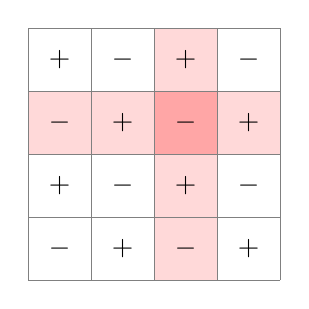
\begin{tikzpicture}[x=0.8cm,y=0.8cm]
  \fill[red!15] (0,2) rectangle (4,3);
  \fill[red!15] (2,0) rectangle (3,4);
  \fill[red!35] (2,2) rectangle (3,3);
  \draw[gray] (0,0) grid[step=1] (4,4);
  \foreach \x/\y in {0.5/3.5,2.5/3.5,1.5/2.5,3.5/2.5,0.5/1.5,2.5/1.5,1.5/0.5,3.5/0.5}{\node at (\x,\y) {$+$};}
  \foreach \x/\y in {1.5/3.5,3.5/3.5,0.5/2.5,2.5/2.5,1.5/1.5,3.5/1.5,0.5/0.5,2.5/0.5}{\node at (\x,\y) {$-$};}
\end{tikzpicture}
\end{center}

\textbf{Figure.} The signs $(-1)^{i+j}$ for a $4\times4$ matrix. The shaded cross is row $2$ and column $3$. Deleting it leaves the $3\times3$ matrix $A_{23}$, and the entry in the darker square sits in a $-$ position, since $2+3=5$ is odd.

\begin{exmp}{A $2\times2$ determinant}{two}
Let $A=\begin{bmatrix}4&-3\\2&5\end{bmatrix}$. Here $A_{11}=[5]$ and $A_{12}=[2]$, so
\[
\det A=4\det[5]-(-3)\det[2]=4\cdot5+3\cdot2=26.
\]
This is $ad-bc=20-(-6)=26$. By Section 2.2 the matrix is invertible, and it carries the unit square to a parallelogram of area $26$.
\end{exmp}

\begin{exmp}{A $3\times3$ determinant along the first row}{threerow}
Let $A=\begin{bmatrix}2&0&3\\1&-2&4\\5&0&-1\end{bmatrix}$. Then
\[
\det A=2\begin{vmatrix}-2&4\\0&-1\end{vmatrix}-0\begin{vmatrix}1&4\\5&-1\end{vmatrix}+3\begin{vmatrix}1&-2\\5&0\end{vmatrix}
=2(2-0)-0+3(0+10)=4+30=34.
\]
The middle term vanished because $a_{12}=0$: we did not even have to compute its minor.
\end{exmp}

\begin{kc}{Signs}{signs}
(a)~Write the checkerboard of signs for a $4\times4$ matrix. (b)~Which sign belongs to the positions $(2,3)$, $(3,1)$, $(4,4)$ and $(3,4)$? (c)~If you expand a $4\times4$ determinant along row~$3$, which signs do the four terms carry? (d)~Suppose $a_{23}=-7$ and $\det A_{23}=3$. What is the number $a_{23}C_{23}$?
\end{kc}

\begin{think}{Why do the signs alternate?}{signs}
(a)~Let $A=\begin{bmatrix}1&2&3\\1&2&3\\0&0&1\end{bmatrix}$. Two equal rows: this matrix is certainly not invertible (Theorem~\ref{2.3-thm:imt}), so a number that detects invertibility had better be $0$. Compute $a_{11}\det A_{11}\pm a_{12}\det A_{12}\pm a_{13}\det A_{13}$ once with the alternating signs $+,-,+$ and once with $+,+,+$. Which choice gives $0$? (b)~Do the same for $\begin{bmatrix}1&1\\1&1\end{bmatrix}$ with signs $+,-$ and $+,+$. (c)~Explain in one sentence why the checkerboard rule $(-1)^{i+j}$ is just the alternating rule applied along a row and along a column.
\end{think}

% ---------------------------------------------------------------------
\subsection*{Any row, any column}

The definition singles out the first row, but the number we want should not depend on a choice of row. The main theorem of this section says that it does not.

\begin{thm}{Cofactor expansion along any row or column}{expansion}
Let $A=[a_{ij}]$ be an $n\times n$ matrix with $n\geq2$. For every row $i$,
\[
\det A=a_{i1}C_{i1}+a_{i2}C_{i2}+\cdots+a_{in}C_{in},
\]
and for every column $j$,
\[
\det A=a_{1j}C_{1j}+a_{2j}C_{2j}+\cdots+a_{nj}C_{nj}.
\]
\end{thm}

\begin{proof}[Proof for $3\times3$ matrices]
We show that every row and every column produces the same six-term sum. Multiplying out the definition (expansion along row $1$) gives
\begin{equation}\label{eq:six}
\det A=a_{11}a_{22}a_{33}-a_{11}a_{23}a_{32}-a_{12}a_{21}a_{33}+a_{12}a_{23}a_{31}+a_{13}a_{21}a_{32}-a_{13}a_{22}a_{31}.
\end{equation}
Now expand along row $2$, whose signs are $-,+,-$:
\begin{align*}
&-a_{21}(a_{12}a_{33}-a_{13}a_{32})+a_{22}(a_{11}a_{33}-a_{13}a_{31})-a_{23}(a_{11}a_{32}-a_{12}a_{31})\\
&\quad=-a_{12}a_{21}a_{33}+a_{13}a_{21}a_{32}+a_{11}a_{22}a_{33}-a_{13}a_{22}a_{31}-a_{11}a_{23}a_{32}+a_{12}a_{23}a_{31}.
\end{align*}
These are the six terms of \eqref{eq:six}, in a different order and with the same signs. Along row $3$, whose signs are $+,-,+$:
\begin{align*}
&a_{31}(a_{12}a_{23}-a_{13}a_{22})-a_{32}(a_{11}a_{23}-a_{13}a_{21})+a_{33}(a_{11}a_{22}-a_{12}a_{21})\\
&\quad=a_{12}a_{23}a_{31}-a_{13}a_{22}a_{31}-a_{11}a_{23}a_{32}+a_{13}a_{21}a_{32}+a_{11}a_{22}a_{33}-a_{12}a_{21}a_{33},
\end{align*}
again the six terms of \eqref{eq:six}. So all three rows give the same number.

For columns, note that the cofactor of $a_{ij}$ in $A$ equals the cofactor of $a_{ji}$ in $A\T$, because deleting row $i$ and column $j$ of $A$ is the same as deleting column $i$ and row $j$ of $A\T$, and a $2\times2$ determinant does not change when its matrix is transposed. Hence the expansion of $A$ down column $j$ is the expansion of $A\T$ along row $j$. Moreover \eqref{eq:six} is unchanged when every $a_{ij}$ is replaced by $a_{ji}$: for example $a_{12}a_{23}a_{31}$ becomes $a_{21}a_{32}a_{13}$, which is the term $a_{13}a_{21}a_{32}$ with the same sign $+$, and the other terms pair up in the same way. So $\det A\T=\det A$, and by the result for rows, expansion of $A\T$ along row $j$ gives $\det A\T=\det A$.
\end{proof}

For $n\geq4$ the theorem is also true. The proof is an induction that uses the same bookkeeping as above; we omit it. From now on we use the theorem freely.

\begin{think}{Why another row cannot change the answer}{otherrow}
(a)~How many products of three entries, one from each row and one from each column, can be formed from a $3\times3$ matrix? How many from a $4\times4$ matrix? (b)~In the proof above, how many terms does the expansion along one row produce? Why does each product appear in it exactly once? (c)~So the three rows can only differ by the \emph{signs} of the six products. Take the product $a_{12}a_{21}a_{33}$ and find its sign when you expand along row $1$ and along row $2$. Why are they equal?
\end{think}

\begin{warn}[Sign trap]
The sign of a term is decided by the \emph{position} of the entry, not by the entry itself, and each row starts with a different sign. Take $M=\begin{bmatrix}1&3&0\\2&-1&4\\0&5&1\end{bmatrix}$. Expansion along row $1$ gives
\[
\det M=1\begin{vmatrix}-1&4\\5&1\end{vmatrix}-3\begin{vmatrix}2&4\\0&1\end{vmatrix}+0=-21-6=-27.
\]
Along row $2$ the signs are $-,+,-$ (the entry $2$ sits in a $-$ position):
\[
\det M=-2\begin{vmatrix}3&0\\5&1\end{vmatrix}+(-1)\begin{vmatrix}1&0\\0&1\end{vmatrix}-4\begin{vmatrix}1&3\\0&5\end{vmatrix}=-6-1-20=-27.
\]
Copying the signs $+,-,+$ of row $1$ onto row $2$ would give $+27$, the right size and the wrong sign, which is easy to miss. Also, the entry $-1$ is in a $+$ position, so its term is $(+)(-1)(1)=-1$: the minus sign of the entry and the minus sign of a position are different things.
\end{warn}

\begin{exmp}{The same matrix along a cleverly chosen column}{threecol}
For the matrix $A=\begin{bmatrix}2&0&3\\1&-2&4\\5&0&-1\end{bmatrix}$ of Example~\ref{ex:threerow}, column $2$ is $(0,-2,0)$. Only the entry $a_{22}=-2$ survives, and it sits in a $+$ position:
\[
\det A=(-2)\,(-1)^{2+2}\begin{vmatrix}2&3\\5&-1\end{vmatrix}=(-2)(-2-15)=34,
\]
the number that the first row gave. One minor instead of two, and no sign trouble.
\end{exmp}

\begin{proc}{Expanding with the fewest terms}{strategy}
\begin{enumerate}
  \item Scan every row and every column for zeros. Choose the line with the most zeros (an entry $\pm1$ is also welcome, since it avoids fractions).
  \item Write down the signs $(-1)^{i+j}$ along that line, starting from the correct position in the checkerboard.
  \item Write only the terms with nonzero entries: entry $\times$ sign $\times$ minor.
  \item Evaluate each smaller determinant in the same way, again looking for its best line.
  \item Combine the terms and re-check the signs. If time allows, check the result along a different line.
\end{enumerate}
\end{proc}

\begin{exmp}{A $4\times4$ determinant with zeros}{fourzeros}
Let $B=\begin{bmatrix}0&2&0&1\\3&1&4&-2\\0&5&0&0\\1&0&2&3\end{bmatrix}$. Row $3$ is $(0,5,0,0)$ and has a single nonzero entry, $b_{32}=5$, in the position $(3,2)$ with sign $(-1)^{3+2}=-$. Hence
\[
\det B=-5\det B_{32}=-5\begin{vmatrix}0&0&1\\3&4&-2\\1&2&3\end{vmatrix}.
\]
In the $3\times3$ determinant, row $1$ has a single nonzero entry $1$ in the position $(1,3)$, sign $+$:
\[
\begin{vmatrix}0&0&1\\3&4&-2\\1&2&3\end{vmatrix}=1\begin{vmatrix}3&4\\1&2\end{vmatrix}=6-4=2.
\]
So $\det B=-5\cdot2=-10$. Two small expansions replaced $4!=24$ products by a handful.
\end{exmp}

\begin{kc}{Compute}{compute}
(a)~$\begin{vmatrix}3&-1\\5&2\end{vmatrix}$. \quad (b)~$\begin{vmatrix}1&2&0\\3&-1&4\\0&5&2\end{vmatrix}$ by expansion along the first row.
\end{kc}

\begin{kc}{Choose the line}{choose}
For each determinant, say which row or column you would expand along and why, and compute it. (a)~$\begin{vmatrix}3&0&-1\\2&0&4\\4&2&7\end{vmatrix}$; \quad (b)~$\begin{vmatrix}1&0&0&2\\0&3&0&0\\4&5&6&7\\0&0&0&8\end{vmatrix}$.
\end{kc}

% ---------------------------------------------------------------------
\subsection*{Triangular matrices and zero lines}

A matrix is \emph{upper triangular} if all entries below the main diagonal are $0$, and \emph{lower triangular} if all entries above it are $0$ (Section 2.3).

\begin{thm}{Triangular matrices}{triangular}
If $A$ is a triangular $n\times n$ matrix, then $\det A$ is the product of the entries on the main diagonal:
\[
\det A=a_{11}a_{22}\cdots a_{nn}.
\]
In particular $\det I_n=1$.
\end{thm}

\begin{proof}
By induction on $n$. For $n=1$ there is nothing to prove. Let $n\geq2$ and assume the result for size $n-1$. If $A$ is upper triangular, the first column is $(a_{11},0,\dots,0)$. Expand down column $1$ (Theorem~\ref{thm:expansion}): the only term is $a_{11}C_{11}=a_{11}\det A_{11}$, and $A_{11}$ is upper triangular of size $n-1$ with diagonal entries $a_{22},\dots,a_{nn}$. By the assumption, $\det A_{11}=a_{22}\cdots a_{nn}$. If $A$ is lower triangular, expand along row~$1$, which is $(a_{11},0,\dots,0)$, in the same way.
\end{proof}

\begin{thm}{A zero row or a zero column}{zero}
If $A$ has a row of zeros or a column of zeros, then $\det A=0$.
\end{thm}

\begin{proof}
Expand along that row or column. Every term has a factor $0$.
\end{proof}

\begin{exmp}{Triangular determinants}{tri}
The upper triangular matrix $T=\begin{bmatrix}2&5&-1&3\\0&-3&4&7\\0&0&1&6\\0&0&0&5\end{bmatrix}$ has $\det T=2\cdot(-3)\cdot1\cdot5=-30$. The lower triangular matrix $L=\begin{bmatrix}3&0&0\\-2&4&0\\7&1&-5\end{bmatrix}$ has $\det L=3\cdot4\cdot(-5)=-60$. The entries off the diagonal play no role at all.

Be careful: the theorem needs a \emph{triangular} matrix. For $N=\begin{bmatrix}0&0&3\\0&2&5\\1&4&6\end{bmatrix}$ the diagonal entries multiply to $0\cdot2\cdot6=0$, but expansion along row $1$ gives $\det N=3\begin{vmatrix}0&2\\1&4\end{vmatrix}=3(0-2)=-6$. The matrix $N$ is triangular only after its rows are put in a different order, and then the diagonal product is not the whole story.
\end{exmp}

\begin{kc}{Triangular}{tri}
Compute the determinant. (a)~$\begin{bmatrix}2&7&1\\0&-1&5\\0&0&3\end{bmatrix}$; \ (b)~$\begin{bmatrix}4&0&0\\1&0&0\\2&3&5\end{bmatrix}$; \ (c)~$\begin{bmatrix}1&2&3&4\\0&1&2&3\\0&0&1&2\\0&0&0&0\end{bmatrix}$. Compare with Theorem~\ref{2.3-thm:triangular}: for which of the three matrices is the determinant nonzero, and which are invertible?
\end{kc}

\begin{think}{Why a product of the diagonal?}{triprod}
(a)~Expand an upper triangular $4\times4$ matrix down its first column, then the $3\times3$ matrix that remains down its first column, and so on. Describe what you see. (b)~Why is expansion along the \emph{first row} the better idea for a lower triangular matrix? (c)~Could you also have expanded a lower triangular matrix down its last column? What would you get?
\end{think}

% ---------------------------------------------------------------------
\subsection*{A parameter, and a $4\times4$ determinant by hand}

\begin{exmp}{For which $h$ is the determinant zero?}{param}
Let $A(h)=\begin{bmatrix}h&3&0\\1&h&2\\0&1&1\end{bmatrix}$. Column $3$ is $(0,2,1)$, with signs $(+,-,+)$, so
\[
\det A(h)=-2\begin{vmatrix}h&3\\0&1\end{vmatrix}+1\begin{vmatrix}h&3\\1&h\end{vmatrix}=-2h+(h^2-3)=h^2-2h-3=(h-3)(h+1).
\]
The determinant is $0$ exactly for $h=3$ and $h=-1$. Now row reduce at these values and at one other. For $h=3$:
\begin{align*}
\begin{bmatrix}3&3&0\\1&3&2\\0&1&1\end{bmatrix}
&\rops{R_1\leftrightarrow R_2}
\begin{bmatrix}1&3&2\\3&3&0\\0&1&1\end{bmatrix}
\rops{R_2-3R_1}
\begin{bmatrix}1&3&2\\0&-6&-6\\0&1&1\end{bmatrix}\\[4pt]
&\rops{-\tfrac16R_2}
\begin{bmatrix}1&3&2\\0&1&1\\0&1&1\end{bmatrix}
\rops{R_3-R_2}
\begin{bmatrix}1&3&2\\0&1&1\\0&0&0\end{bmatrix}.
\end{align*}
For $h=-1$:
\begin{align*}
\begin{bmatrix}-1&3&0\\1&-1&2\\0&1&1\end{bmatrix}
&\rops{R_2+R_1}
\begin{bmatrix}-1&3&0\\0&2&2\\0&1&1\end{bmatrix}
\rops{R_3-\tfrac12R_2}
\begin{bmatrix}-1&3&0\\0&2&2\\0&0&0\end{bmatrix}.
\end{align*}
Both matrices have only two pivots, so by Theorem~\ref{2.3-thm:imt} they are singular. For $h=0$ the determinant is $(0-3)(0+1)=-3\neq0$ and $A(0)=\begin{bmatrix}0&3&0\\1&0&2\\0&1&1\end{bmatrix}$ has three pivots (rows $2,1,3$ in that order are already in echelon form). In all three cases the determinant is zero exactly when the matrix is singular, as the discussion at the beginning of this section led us to expect.
\end{exmp}

\begin{exmp}{A $4\times4$ determinant by hand}{fourhand}
Let $C=\begin{bmatrix}1&2&0&3\\2&1&1&0\\0&3&1&2\\1&0&2&1\end{bmatrix}$. There is no row or column with more than one zero, so choose row $1$, which has a zero in the third position. Then $\det C=1\cdot M_{11}-2M_{12}+0-3M_{14}$ with $M_{1j}=\det C_{1j}$:
\begin{align*}
M_{11}&=\begin{vmatrix}1&1&0\\3&1&2\\0&2&1\end{vmatrix}=1(1-4)-1(3-0)+0=-6,\\
M_{12}&=\begin{vmatrix}2&1&0\\0&1&2\\1&2&1\end{vmatrix}=2(1-4)-1(0-2)+0=-4,\\
M_{14}&=\begin{vmatrix}2&1&1\\0&3&1\\1&0&2\end{vmatrix}=2(6-0)-1(0-1)+1(0-3)=10.
\end{align*}
Hence $\det C=1(-6)-2(-4)-3(10)=-6+8-30=-28$.

\textbf{Check along column $1$} (signs $+,-,+,-$; the third entry is $0$): the minors are $M_{11}=-6$, $M_{21}=\begin{vmatrix}2&0&3\\3&1&2\\0&2&1\end{vmatrix}=12$ and $M_{41}=\begin{vmatrix}2&0&3\\1&1&0\\3&1&2\end{vmatrix}=-2$, so $\det C=1(-6)-2(12)+0-1(-2)=-6-24+2=-28$. Two different lines, the same number.
\end{exmp}

\begin{kc}{A parameter}{param}
Let $D(h)=\begin{bmatrix}2&h&0\\1&3&h\\0&1&1\end{bmatrix}$. For which $h$ is $\det D(h)=0$? For that $h$ row reduce $D(h)$ and count the pivots.
\end{kc}

% ---------------------------------------------------------------------
\subsection*{How practical is cofactor expansion?}

\begin{warn}[A shortcut that fails]
You may have seen a trick for $3\times3$ determinants: copy the first two columns to the right of the matrix and add and subtract products along six diagonals. It produces exactly the six terms of \eqref{eq:six} and nothing else, so it cannot be extended. A $4\times4$ determinant has $4!=24$ terms but this trick yields only $8$ diagonal products. Applied to a $4\times4$ matrix it gives wrong answers. We do not use it. Cofactor expansion works for every size.
\end{warn}

\begin{exmp}{How many multiplications?}{cost}
Let $m(n)$ be the number of multiplications used by cofactor expansion of an $n\times n$ determinant along the first row, if no entry is zero. For $n=2$ we need $m(2)=2$ products. For $n\geq3$ we must evaluate $n$ determinants of size $n-1$ and then multiply each of them by an entry, so $m(n)=n\,m(n-1)+n$, which is more than $n\,m(n-1)$. By induction $m(n)>n!$ for $n\geq3$. Some values: $10!=3{,}628{,}800$ and $25!\approx1.55\times10^{25}$. A computer that performs $10^{12}$ multiplications per second would need $1.55\times10^{13}$ seconds, almost $500{,}000$ years, for one $25\times25$ determinant. Cofactor expansion is a tool for small matrices and for matrices with many zeros.
\end{exmp}

\begin{think}{Can we do better?}{faster}
(a)~Check on $\begin{bmatrix}1&2\\3&4\end{bmatrix}$ and on the matrices you get after each of the three elementary row operations (a replacement $R_2-3R_1$, an interchange, a scaling $2R_1$) how the determinant changes. (b)~Which row operations would make cofactor expansion cheap? (c)~How would you finish if you managed to reach a triangular matrix?
\end{think}

\begin{think}{A matrix with zeros everywhere you want them}{zerosplace}
(a)~A $5\times5$ matrix has exactly one nonzero entry in each row and each column (a permutation-type matrix). Using the strategy above, how many products does the expansion need? (b)~What can you say about its determinant compared with $1$? Test on $\begin{bmatrix}0&1&0\\0&0&1\\1&0&0\end{bmatrix}$ and $\begin{bmatrix}0&1\\1&0\end{bmatrix}$.
\end{think}

\subsection*{Summary}
\begin{itemize}
  \item Row reduction of a $3\times3$ matrix with $a_{11}\neq0$ and $p\neq0$ produces the pivots $a_{11},\ p,\ a_{11}\Delta$ with $\Delta$ as in \eqref{eq:delta}: the matrix has three pivots exactly when $\Delta\neq0$.
  \item $\det[a]=a$; for $n\geq2$, $\det A=\sum_j(-1)^{1+j}a_{1j}\det A_{1j}$ (recursive definition). For $2\times2$ it is $ad-bc$.
  \item The $(i,j)$-cofactor is $C_{ij}=(-1)^{i+j}\det A_{ij}$; the signs form a checkerboard starting with $+$. \textbf{The sign belongs to the position, not to the entry.}
  \item \textbf{Cofactor expansion along any row or any column} gives the same number. Choose the line with the most zeros.
  \item The determinant of a \textbf{triangular} matrix is the product of its diagonal entries; a matrix with a zero row or zero column has determinant $0$.
  \item In the examples of this section, $\det A=0$ exactly when $A$ is singular. For triangular matrices this follows from Theorem~\ref{2.3-thm:triangular}.
  \item Cofactor expansion needs more than $n!$ multiplications. It is not a method for large matrices. The trick of copying columns works only for $3\times3$.
\end{itemize}

\subsection*{Questions to think about before the next section}
\begin{enumerate}
  \item Cofactor expansion is far too slow for large matrices, but row reduction is fast. What happens to the determinant of a $2\times2$ matrix when you do one row operation? Try the three kinds and guess what happens for larger matrices.
  \item In every example so far $\det A=0$ exactly when $A$ is singular, and for triangular matrices we know why. Is this true for \emph{every} square matrix? How could we prove it, using only what we know about row reduction?
  \item The number $|ad-bc|$ measures an area. What should $|\det A|$ measure for a $3\times3$ matrix?
\end{enumerate}

\subsection*{Answers and discussion}
\begin{description}[leftmargin=0pt,itemsep=5pt]
  \item[Knowledge Check \ref{kc:signs}.] (a)~$\begin{bmatrix}+&-&+&-\\-&+&-&+\\+&-&+&-\\-&+&-&+\end{bmatrix}$. (b)~$(2,3)$: $-$ (since $2+3=5$ is odd); $(3,1)$: $+$; $(4,4)$: $+$; $(3,4)$: $-$. (c)~Row $3$ of the checkerboard is $+,-,+,-$, so the terms carry the signs $+,-,+,-$. (d)~$C_{23}=(-1)^{2+3}\cdot3=-3$, so $a_{23}C_{23}=(-7)(-3)=21$.
  \item[Knowledge Check \ref{kc:compute}.] (a)~$3\cdot2-(-1)\cdot5=6+5=11$. (b)~$1\begin{vmatrix}-1&4\\5&2\end{vmatrix}-2\begin{vmatrix}3&4\\0&2\end{vmatrix}+0=1(-2-20)-2(6-0)=-22-12=-34$.
  \item[Knowledge Check \ref{kc:choose}.] (a)~Column $2$ is $(0,0,2)$: expand down it, only $a_{32}=2$ survives, with sign $(-1)^{3+2}=-$: $-2\begin{vmatrix}3&-1\\2&4\end{vmatrix}=-2(12+2)=-28$. (b)~Row $2$ is $(0,3,0,0)$: the entry $3$ is in position $(2,2)$, sign $+$, so $\det=3\begin{vmatrix}1&0&2\\4&6&7\\0&0&8\end{vmatrix}$. In that $3\times3$ determinant row $3$ is $(0,0,8)$ with sign $+$ at position $(3,3)$: $8\begin{vmatrix}1&0\\4&6\end{vmatrix}=8\cdot6=48$. So the determinant is $3\cdot48=144$.
  \item[Knowledge Check \ref{kc:tri}.] (a)~$2\cdot(-1)\cdot3=-6$. (b)~$4\cdot0\cdot5=0$. (c)~$1\cdot1\cdot1\cdot0=0$ (also a zero row). The determinant is nonzero only for~(a). By Theorem~\ref{2.3-thm:triangular} the matrix in~(a) is invertible and those in~(b) and~(c) are singular, because they have a zero on the diagonal. For triangular matrices, $\det A\neq0$ and ``$A$ invertible'' say the same thing.
  \item[Knowledge Check \ref{kc:param}.] Expand down column $3$, whose entries are $0,h,1$ with signs $+,-,+$: $\det D(h)=-h\begin{vmatrix}2&h\\0&1\end{vmatrix}+1\begin{vmatrix}2&h\\1&3\end{vmatrix}=-2h+(6-h)=6-3h$. This is $0$ exactly for $h=2$. Then $D(2)=\begin{bmatrix}2&2&0\\1&3&2\\0&1&1\end{bmatrix}$, and
  \begin{align*}
  \begin{bmatrix}2&2&0\\1&3&2\\0&1&1\end{bmatrix}
  &\rops{R_2-\tfrac12R_1}
  \begin{bmatrix}2&2&0\\0&2&2\\0&1&1\end{bmatrix}
  \rops{R_3-\tfrac12R_2}
  \begin{bmatrix}2&2&0\\0&2&2\\0&0&0\end{bmatrix}
  \end{align*}
  has two pivots, so $D(2)$ is singular.
  \item[Pause and think \ref{think:numberwant}.] (a)~The natural value is $abc$, the product of the diagonal entries. Formula \eqref{eq:delta} gives $a(bc-0)-0+0=abc$. (b)~A matrix with a row of zeros has fewer than three pivots, so it is singular and the number must be $0$. In the expanded form of \eqref{eq:delta} (the six terms of \eqref{eq:six}), every term contains exactly one entry from each row, so every term contains an entry of the zero row and vanishes.
  \item[Pause and think \ref{think:signs}.] (a)~The minors are $\det A_{11}=\begin{vmatrix}2&3\\0&1\end{vmatrix}=2$, $\det A_{12}=\begin{vmatrix}1&3\\0&1\end{vmatrix}=1$, $\det A_{13}=\begin{vmatrix}1&2\\0&0\end{vmatrix}=0$. With $+,-,+$: $1\cdot2-2\cdot1+3\cdot0=0$. With $+,+,+$: $2+2+0=4\neq0$. Only the alternating signs give $0$, as they must for a matrix with two equal rows. (b)~With $+,-$: $1\cdot1-1\cdot1=0$; with $+,+$: $1+1=2$. (c)~Alternating signs along a row, and also down a column, mean that the sign of position $(i,j)$ changes whenever $i$ or $j$ changes by one, that is $(-1)^{i+j}$.
  \item[Pause and think \ref{think:otherrow}.] (a)~$3!=6$ and $4!=24$: choose the entry from row $1$ in any of $n$ columns, then from row $2$ in any of the $n-1$ remaining columns, and so on. (b)~Six terms: three entries of the chosen row, times the two products of the $2\times2$ determinant that is left. A product $a_{1i}a_{2j}a_{3k}$ uses exactly one entry of the chosen row, say $a_{2j}$, and then the other two entries are a term of the $2\times2$ minor of that entry, so it occurs once. (c)~Along row $1$: the entry $a_{12}$ is in a $-$ position and the remaining product $a_{21}a_{33}$ occurs in the minor with a $+$ sign (it is the product of the main diagonal), so the sign is $-$. Along row $2$: the entry $a_{21}$ is in a $-$ position and the remaining product $a_{12}a_{33}$ is the main diagonal product of its minor, so again $-$. The checkerboard is exactly the rule that makes these signs agree.
  \item[Pause and think \ref{think:triprod}.] (a)~Each time the first column has a single nonzero entry on top, so the determinant is $a_{11}$ times the determinant of the matrix obtained by deleting row $1$ and column $1$; that matrix is again upper triangular. After four steps we get $a_{11}a_{22}a_{33}a_{44}$. (b)~Row $1$ of a lower triangular matrix is $(a_{11},0,\dots,0)$: one term. (c)~Yes. The last column of a lower triangular matrix is $(0,\dots,0,a_{nn})$ with the sign $(-1)^{n+n}=+$, and what remains is again lower triangular, giving the same product. By Theorem~\ref{thm:expansion} any row or column may be used.
  \item[Pause and think \ref{think:faster}.] (a)~For $A=\begin{bmatrix}1&2\\3&4\end{bmatrix}$, $\det A=-2$. Replacement $R_2-3R_1$: $\begin{bmatrix}1&2\\0&-2\end{bmatrix}$, $\det=-2$, unchanged. Interchange: $\begin{bmatrix}3&4\\1&2\end{bmatrix}$, $\det=2$, the sign is reversed. Scaling $2R_1$: $\begin{bmatrix}2&4\\3&4\end{bmatrix}$, $\det=-4$, multiplied by $2$. (b)~Replacements that create zeros in a column (they appear to leave the determinant unchanged), so that an expansion has a single term. (c)~Multiply the diagonal entries (Theorem~\ref{thm:triangular}), correcting for whatever the operations did to the determinant.
  \item[Pause and think \ref{think:zerosplace}.] (a)~Each expansion has a single nonzero term, so the sizes shrink $5,4,3,2,1$ with one product each; no matter which line you choose the answer is a single product of the $5$ nonzero entries, up to a sign. (b)~The determinant is $\pm$ the product of the nonzero entries. For the $3\times3$ matrix, expanding along column $1$ (only $a_{31}=1$, sign $+$) gives $1\begin{vmatrix}1&0\\0&1\end{vmatrix}=1$. For $\begin{bmatrix}0&1\\1&0\end{bmatrix}$: $0-1=-1$. The sign records how the ones are arranged, whether the rows have to be interchanged an odd or an even number of times to reach $I$.
  \item[Before the next section.] (1)~For $\begin{bmatrix}1&2\\3&4\end{bmatrix}$ we found: replacement leaves $\det$ unchanged, interchange reverses its sign, scaling a row by $c$ multiplies it by $c$ (Pause and think \ref{think:faster}). The guess is that this holds for any size. (2)~Yes, it is true, and the proof will combine the effect of row operations on the determinant with the fact that a square matrix is invertible exactly when row reduction produces $n$ pivots. (3)~The volume of the parallelepiped spanned by the columns, that is, the volume of the image of the unit cube.
\end{description}

\end{document}
